\section{SCGRA Overlay Infrastructure} \label{sec:scgraimplement}
One key idea of QuickDough is to rely on an intermediate SCGRA overlay to improve compilation time of the high-level user application. While the exact design of this SCGRA does not affect the compilation flow, its implementation does have a significant impact on the performance of the generated gateware.
 
\subsection{SCGRA Based FPGA Accelerator}
Figure \ref{fig:scgra-accelerator} is the proposed FPGA accelerator built on top of the SCGRA overlay. The input/output data buffers and Acc Ctrl block are almost the same with those in the typical acceleration architecture \ref{fig:typical-FPGA-accelerator}, while the rest blocks are unique. 

Particularly, the kernel part of the accelerator is a synchronous 2D torus SCGRA which consists of an array of PEs. Details of the PE will be illustrated in the next section. Another major difference is that two address buffers instead of the customized logic are used as the address generator to control the on-chip buffer accessing. With the address buffers, there is no need to develop any spcific address generator when the target application changes, as we can simply replace its content together with the SCGRA configuration memory according to the scheduling result. Therefore, it reduces the chance of FPGA implementation and is beneficial to improving the design productivity. 

Finally, it is noted that input and output data buffers could accommodate more data than that used by a single SCGRA execution, so the SCGRA may iterate multiple times before it consumes all the data in input buffer or fills the output buffer. From the perspective of host processor, it is more efficient to control multiple SCGRA execution at a time instead of each SCGRA execution independently. In this case, we have a control unit called SCGRA Ctrl to make the multiple SCGRA execution transparent to the Acc Ctrl. Also sharing the data sets among multiple SCGRA execution could make best use of the limited input/output buffer. In addition, the regular SCGRA overlay tends to run at higher frequency than the data buffer controller handling the system bus protocol, and two sets of synchronous registers are added to keep the computation core and the rest of the design to running at individual clock domains.  

\begin{figure}[h]
    \center{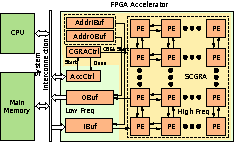
\includegraphics[width=0.8\linewidth]{scgra-accelerator}}
    \caption{SCGRA Accelerator}
    \label{fig:scgra-accelerator}
\end{figure}

\subsection{PE}
In this section, an instance of PE is presented to demonstrate the feasibility of producing high performance gateware. As shown in \figref{fig:pe}, the PE, centring an ALU block, a multiple-port data memory and an instruction memory, is highly optimized for FPGA implementation. In addition, load/store paths are implemented on the PEs that are responsible for data I/O beyond the FPGA. Addr Ctrl is used to start and reset the SCGRA execution by changing the instruction memory read address sequentially, so it has a single bit global start input signal from the SCGRA Ctrl block. 

\begin{figure}[h]
\center{\includegraphics[width=0.95\linewidth]{pe}}
\caption{PE structure}
\label{fig:pe}
\end{figure}

\subsubsection{Instruction Memory and Data Memory}
The instruction memory stores all the control words of the PE in each cycle. Since its content does not change during runtime, a ROM is used to implement this instruction memory and the content of the ROM can be loaded directly into a pre-implemented bitstream. The address of the instruction ROM is determined by the Addr Ctrl. Basically, the SCGRA execution will proceed sequentially when the start signal is valid, and it will be reset when the start signal is invalid.

Data memory stores intermediate data that can either be forwarded to the PE downstream or be sent to the ALU for calculation. For fully parallelized operation, \emph{at least} four read ports are needed -- three for the ALU and one for data forwarding. Similarly, at least two write ports are needed to store input data from upstream memory and to store the result of the ALU in the same cycle. Although a pair of true dual port memories seem to meet this port requirement, conflicts may arise if the ALU needs to read the data while the data path needs to be written. As a result, a third dual port memory is replicated in the data memory.

Note that data memory here is usually implemented using a multiple port register file in many previous CGRA work. Although register file is even more flexible in terms of parallel reading and writing, the multi-port register file size is limited due to the inefficient hardware implementation. While we have a much larger DFG for scheduling and thus larger temporary storage is required, eventually a multi-port data memory is used instead. 

\subsubsection{ALU}
At the heart of the proposed PE is an ALU designed to cover the computations in target application. \figref{fig:ALU} shows an example design that could support all the operations of our benchmark which is listed in \tabref{tab:operations}. Complex operations like MULADD/MULSUB are implemented with DSP core directly. Operations with moderate complexity like ADDADD, RSFAND etc. are divided into two stages naturally and hardware block reuse is also considered at the same time. Finally, simple operations that can be done in a single cycle can be put in either stage depending on the pipeline status. Note that MUX in data path has significant influence on timing as well, so small MUX should be inserted properly and large MUX should be avoided. Currently, we just manually create the ALU design, but it is possible to automate this step. 

\begin{figure}[h]
\center{\includegraphics[width=0.8\linewidth]{alu}}
\caption{ALU Example}
\label{fig:ALU}
\end{figure} 

\begin{table}[h]
\caption{Operation Set Implemented in ALU}
\label{tab:operations}
\centering
\begin{tabular}{|p{1.5cm}|p{1.5cm}|p{4cm}|}
\hline
Type & Opcode & Expression \\

\hline
MULADD & 0001 & {dst = src0 $\times$ src1 + src2} \\

\hline
MULSUB & 0010 & {dst = src0 $\times$ src1 - src2} \\

\hline
ADDADD & 0011 & {dst = src0 + src1 + src2} \\

\hline
ADDSUB & 0100 & {dst = src0 + src1 - src2} \\

\hline
SUBSUB & 0101 & {dst = src0 - src1 - src2} \\

\hline 
PHI & 0110 & {dst = src0 ? src1 : src2} \\

\hline
RSFAND & 0111 & {dst = (src0 $\gg$ src1) \& src2} \\

\hline
LSFADD & 1000 & {dst = (src0 $\ll$ src1) + src2} \\

\hline
ABS & 1001 & {dst = abs(src0)} \\

\hline
GT & 1010 & {dst = (src0 $>$ src1) ? 1 : 0} \\

\hline
LET & 1011 & {dst = (src0 $\leq$ src1) ? 1 : 0} \\

\hline
ANDAND & 1100 & {dst = src0 \& src1 \& src2} \\

\hline
\end{tabular}
\end{table}

\subsection{Load/Store Interface}
For the PEs that also serve as IO interface to the SCGRA, they have additional load path and store path as shown in \ref{fig:pe}. Load path and the SCGRA neighboring input share a single data memory write port, and an additional pipeline stage is added to keep the balance of the pipeline. Store path has an additional data MUX as well, but it doesn't have significant influence on the rest of the design. 

